\subsection{Banktilgang}
\begin{figure}[!htb]
\centering
\begin{minipage}{0.4\textwidth}
	Det første du må gjøre, er å levere inn en egenerklæring til økonomiansvarlig i HS. Det ligger et skjema på ntnui.no som fylles ut med kopi av gyldig legitimasjon. Se gjerne bildet til høyre. \\
	Deretter må du besøke \href{https://www.danskebank.no/nb-no/bedrift/smaabedrifter/nettbank/pages/identifisering.aspx}{danskebank.no og legitimere deg med BankID}. Den enkleste måten å finne frem på, er å google \emph{``danske bank legitimering''}. \\ \\
Når alt det er gjort, vil økonomiansvarlig opprette en bruker hos banken, og du vil finne kodebrikke og midlertidig passord i posthylla etter 3-4 virkedager.
\end{minipage}
\begin{minipage}{0.5\textwidth}
	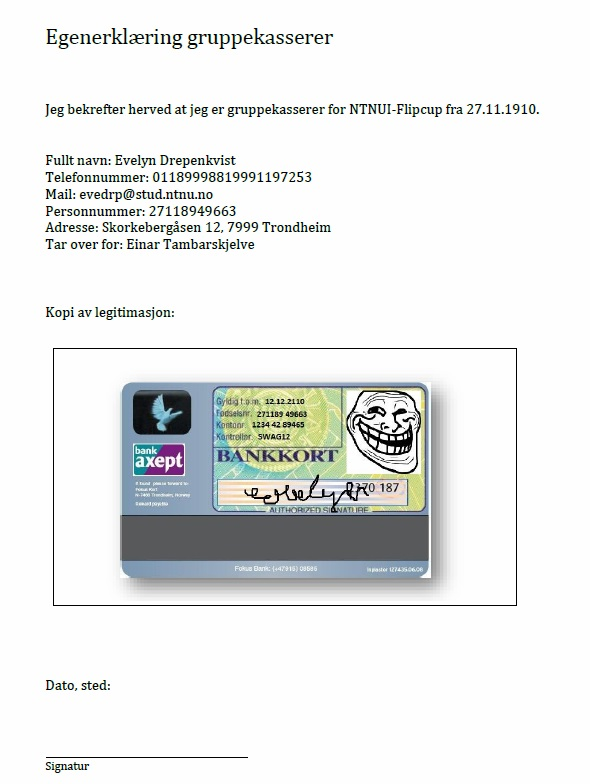
\includegraphics[scale=0.5]{bildr/egenerklaring.jpg}
\end{minipage}
\end{figure}

\subsection{God praksis}
Gjennom arbeidet ditt er det viktig å huske at det du gjør er del av et større regnskap, og det er derfor viktig at alle gruppene følger de samme grunnleggende prinsippene, og at man er konsekvent i praksis i hele foreningen. Det er en stor plass for egenart i føringa, men den kan ikke avvike for langt fra det som er praksis i resten av foreninga, så kommentarer fra hovedkasserer er å anse som ufravikelige instrukser, og er aldri ment som direkte kritikk mot arbeidet ditt, men som nødvendige endringer for å holde seg innafor god skikk i foreningen. Dialog er derfor veldig viktig, og du bør aldri nøle med å kontakte foreningens hovedkasserer for å spørre om råd.

\subsubsection*{Par kjappe tips}
og nå, noen kjappe tips!

\begin{description}
\item [Forfallsdato på innbetalinger] Nyttig vane er å kreve mer fra medlemmene dine! Konsekvent praksis gjør livet ditt enklere. F.eks kan man slå sammen posteringa i bilaget mot innbetalingene på konto hvis de skjer på samme dag (på norsk: du kan slå sammen summen av innbetalingene til en post mot 1920 hvis alle er samme dato). Minn medlemmene dine på at de kan sette forfallsdato på utbetalingene, og bli enige om hvilken dag som er best for {\bfseries deg}.
\item[Fått inkassokrav?] Ring til inkassobyrået med en gang! Kravet ligger hos de, så ikke stress med å kontakte leverandør med en gang. Er kravet allerede gjort opp? Forklar det. Det viktigste er å få inkassokravet satt på hold, og de fleste byrå er veldig greie å ha med hvis du bare tar kontakt og starter dialogen med en gang. Det er generelt lite gøy å tape penger over dust høye renter og gebyr.
\item[Reiseregninger] Reiseregninger er lett en av de mest knotete greiene du kommer borti. Gjør livet ditt enklere og dytt litt av ansvaret over på medlemmene. Sørg for at lag har en reiseansvarlig, og krev at reiseansvarlig leverer reiseregningen pent og pyntelig med all nødvendig dokumentasjon allerede samlet sammen (boardingkort, kvitteringer på billetter, bensin, bompenger, ol.). Gjør livet \emph{ditt} lettere. Vær også gjerne unødig bastant og nekt å betale ut eller ta i mot reiseregninger før de er samlet sammen skikkelig. Det er ditt ansvar for at det for enhver utbetaling er tilstrekkelig dokumentasjon, så du er i din fulle rett til å nekte å betale ut refusjon skulle dokumentasjon utebli.
\item[Generelt om leverandørgjeld] Hva med likheten i postadressen mellom \emph{NTNU} og \emph{NTNUI} skjer det titt og ofte at fordringer sendes til feil adresse. Dette er \emph{deres} feil, også selv om det er ditt problem at kravet ikke er gjort opp. Uansett er dette et stort punkt å krangle på hvis kravet skulle gå til inkasso fordi fakturaen er feiladressert. Å følge opp sånne småting kunne lett ha spart flere grupper unødige gebyr.
\end{description}
